\documentclass[../main.tex]{subfiles}

\begin{document}

\section{10.2 - Optimal Control of Pitch/Travel without Feedback}

\subsection{Derivation of a continous time state space model}
In this part of the exercise we will disregard elevation, therefore we assume $ e = 0 $ and do include it in the model.

The state-vector, $\bm x$ is defined as:
\begin{equation}\label{eq:lab2_state}
	\bm x = 
	\begin{bmatrix}
		\lambda & r & p & \dot p
	\end{bmatrix}
	^T ,
\end{equation}
where $\lambda$ is travel, $r$ is speed of travel (travelrate), $p$ is pitch and $\dot{p}$ is pitchrate.

The dynamic equations for the system was given in the problem description. The following equations were given:
\begin{subequations} 
	\begin{align}
		\dot \lambda &= r \\
		\dot r &= -K_2 p, \quad K_2 = \frac{K_p l_a}{J_t}\\
		\dot p &= \dot p \\
		\ddot p &= -K_1 K_{pd} \dot p - K_1 K_{pp} p + K_1 K_{pp} pc, \quad K_1 = \frac{K_f l_h}{J_p}
	\end{align}
\end{subequations}
The state-space form of the system therefore becomes: 
\begin{equation}\label{eq:lab2_cont_ss}
	\underbrace{\begin{bmatrix}
		\dot \lambda \\
		\dot r \\
		\dot p \\
		\ddot p
	\end{bmatrix}}_{\bm{\dot x}} = 
	\underbrace{
	\begin{bmatrix}
		0 & 1 & 0 & 0 \\
		0 & 0 & -K_2 & 0 \\
		0 & 0 & 0 & 1 \\
		0 & 0 & -K_1 K_{pp} &  -K_1 K_{pd}
	\end{bmatrix}
	}_{\bm A_c}
	\begin{bmatrix}
		\lambda \\ r \\ p \\ \dot{p} \\
	\end{bmatrix}
	+
	\underbrace{
		\begin{bmatrix}
			0 \\ 0 \\ 0 \\ K_1 K_{pp}
		\end{bmatrix}
	}_{\bm B_c} \underbrace{p_c}_{u}
\end{equation}

\subsubsection{Stability and eigenvalues}
The properties of this system is dependent on physical constants ($l_a, J_t, ...$) and control parameters ($K_{pp}, K_{pd}$).

Symbolic expressions in Matlab shows that the eigenvalues of A are:
\begin{equation}
	\lambda = \pm \frac{1}{2} \left( \sqrt{-K_1 (-K_1 K_{pd}^2 + 4  K_{pp})} - K_1  K_{pd} \right)
\end{equation}

The eigenvalues of the continous model, with $K_{pp} = 0,1 , K_{pd} = 0,4$ are:
\begin{equation}\label{eq:lab2_ss_c_eigenvalues_example}
	\begin{bmatrix}
		0 \\ 0 \\ -0.26 + 0.24i \\ -0.26 - 0.24 \\
	\end{bmatrix}
\end{equation}

\todo{Make a plot showing stability dependent on control parameters? Or an analytical description.}



\subsection{The discretized model}
\textit{Answer 10.2.1.2. Remember to document the calculations.} \todo{Remove} \\
\subsubsection{Discretizing model}
Forward Euler method is given by:
\begin{equation}\label{eq:lab2_forward_euler}
	\bm{x}[k + 1] = \bm I \bm x[k] + T\bm{A_c x}[k] + T\bm B_c
\end{equation}, where $ T $ is the timestep \todo[inline]{timestep in the discretization??}\todo[inline]{Add reference to linsys slides}.
Reformulating this, we can write:
\begin{equation}\label{eq:lab2_discrete_system}
	\bm{x}_{k + 1} = \underbrace{(\bm I + T \bm A_c)}_{\bm A} \bm{x}_{k} + \underbrace{T \bm B_c}_{\bm B} u_k
\end{equation}

\subsubsection{Checking stability}
The stability condition for \cref{eq:lab2_discrete_system} is:
\begin{equation}\label{eq:lab2_stab_condition}
	|1 + T \lambda| \leq 1
\end{equation}, where $ \lambda $ is an eigenvalue of $ \bm A_c $ in \cref{eq:lab2_discrete_system}. 
\todo[inline]{Where is this equation from? I believe that it works, but we should either derive it or reference where we found it. ANSWER: From linsys slides, see above}
Using MATLAB we found the eigenvalues of $ \bm A $ to be ... \todo[inline]{Add Matlab appendix}
\todo[inline]{find eigenvalues}

\subsection{The open loop optimization problem}
\textit{How is it formulated?}

\subsection{The weights of the optimization problem}
\textit{Try using the values 0.1, 1 and 10 as weights q. Plot the manipulated variable and the output. Comment the results with respect to the different weights chosen.}
% TODO: \usepackage{graphicx} required
\begin{figure}
	\centering
	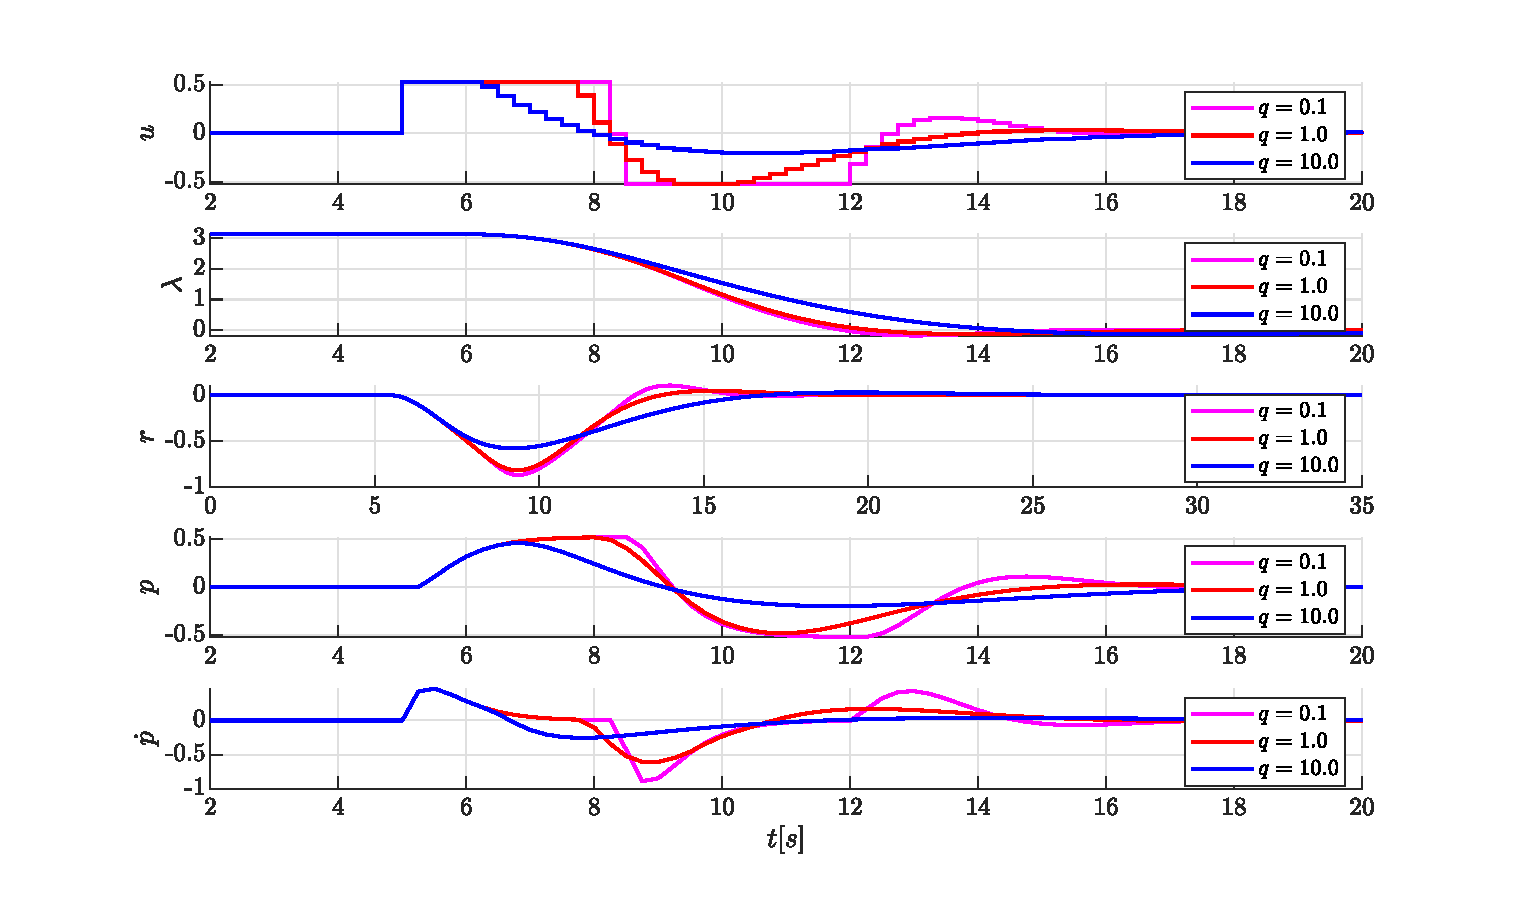
\includegraphics[width=\linewidth]{figures/lab2_optimal_u}
	\caption{Manipulated variable and outputs with different values of $q$.}
	\label{fig:lab2optimalu}
\end{figure}

\subsection{The objective function}
\textit{Furthermore, discuss the objective function (15) (in the lab assignment text) in particular the term $(\lambda_i-\lambda_f )^2$. For instance, could any unwanted effects arise from steering the helicopter to $\lambda =\lambda_f$ with this objective function?}

\subsection{Experimental results}
\textit{Printouts of data from relevant experiments (plots).
Discussion and analysis of the results.
Answer 10.2.2.7 here.}

\subsection{MATLAB and Simulink}
\textit{Code and diagrams go here}
	
\end{document}